\chapter{Compute architecture and scheduling}
\begin{center}
    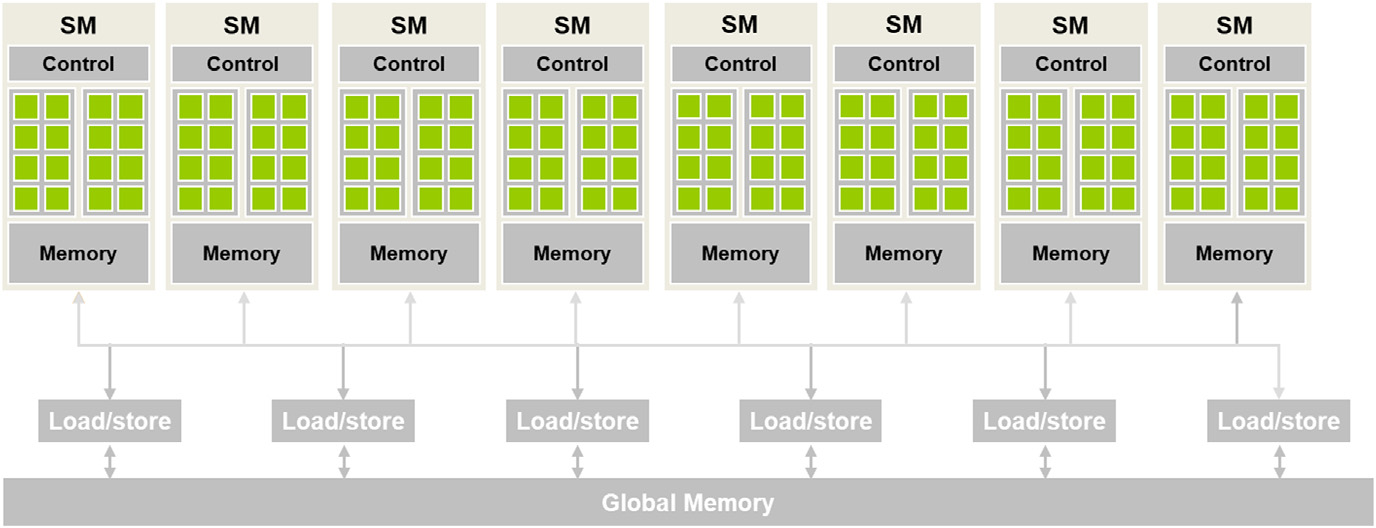
\includegraphics[width=0.7\linewidth]{Images/CompArch/CUDA_GPU.png}
\end{center}
\begin{itemize}
    \item A CUDA capable GPU is organized into an array of highly threaded streaming multiprocessors(SMs).
          \begin{itemize}
              \item Each SM $\rightarrow$ has several processing units called CUDA Cores (cores).
                    \begin{itemize}
                        \item Each Core $\rightarrow$ shares control logic and memory resources.
                    \end{itemize}
          \end{itemize}
\end{itemize}

\section{Block scheduling}
\begin{center}
    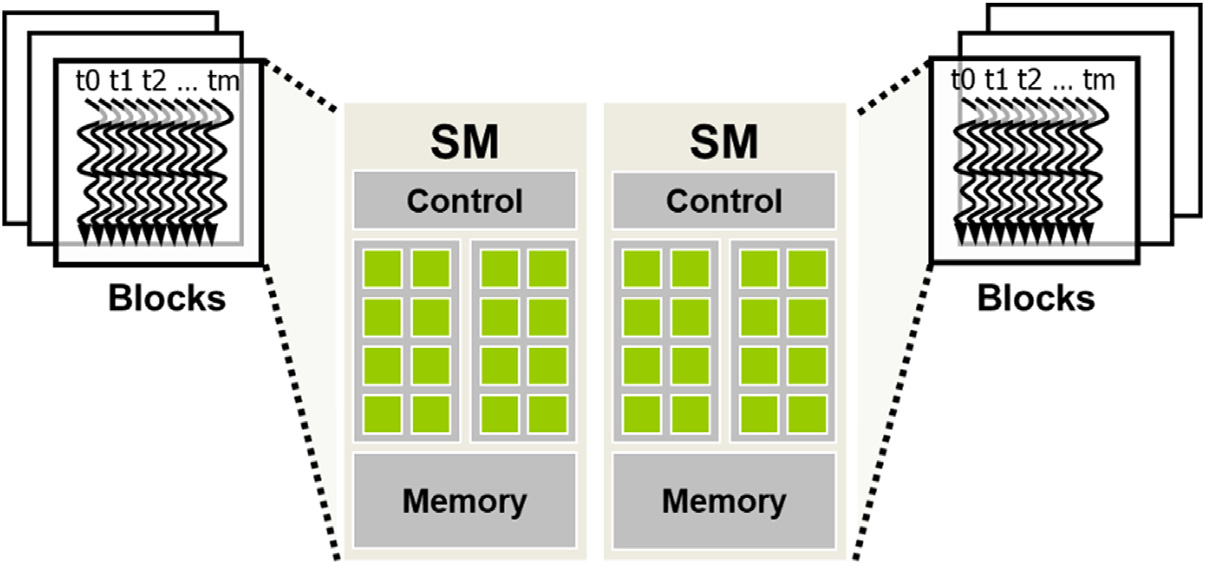
\includegraphics[width=0.7\linewidth]{Images/CompArch/block_assignment.png}
\end{center}
When the kernel is called, the CUDA runtime system launches a grid of threads that execute kernel code. The threads are attached to Streaming Multiprocessors (SMs) on a block-by-block basis.
\begin{itemize}
    \item i.e, \textbf{all the threads in a block are assigned to the same SM}.
    \item Multiple blocks are assigned to the same SM.
    \item \textbf{Blocks need to reserve hardware resources} to execute. $\implies$ A \textbf{limited number of blocks can be assigned to an SM.}
          \begin{itemize}
              \item As the \textbf{number of SMs} in a GPU is \textbf{limited}, the \textbf{total number of blocks that can be simultaneously executing on a CUDA device is limited}.
              \item Most grids contain many more blocks than this number. To ensure all the blocks in a grid get executed, the runtime system maintains a list of blocks that need to execute and assigns new blocks to SMs when previously assigned blocks complete execution.
          \end{itemize}
    \item This fashion of assignment of threads to SMs \textbf{guarantees that the threads in the same block are scheduled simultaneously on the same SM}. This \textbf{guarantee enables the threads in the same block to interact with each other} in ways that the threads across the blocks cannot.
\end{itemize}

\section{Synchronization and transparent scalability}
\subsection{\_\_syncthreads()}
\begin{itemize}
    \item The threads from the same block can coordinate their activities using the barrier synchronization function \texttt{\_\_syncthreads()}.
    \item If a thread calls \texttt{\_\_syncthreads()}, the thread will be held at the program location of the call, until all threads in the block reach that location. Ensures all the threads have completed a phase of their execution before moving to the next phase.
          \begin{center}
              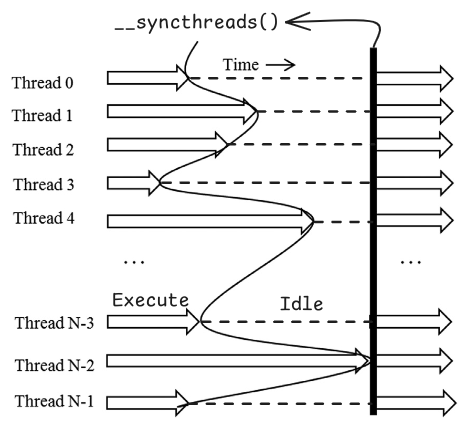
\includegraphics[width=0.7\linewidth]{Images/CompArch/syncthreads.png}
          \end{center}
    \item Among the \textsl{N threads} in the image above, the $\textsl{N-2 }^{nd}$ thread is the last to execute. But all the other threads wait for the $\textsl{N-2 }^{nd}$ thread to finish the execution, thus ensuring the same program location / state among all the threads in the block.
    \item With barrier synchronization, \enquote{no one is left behind.}
    \item In CUDA, if a \textbf{\texttt{\_\_syncthreads()}} statement is present, it \textbf{must be executed by all threads in a block}.
    \item \textbf{\texttt{\_\_syncthreads()}} in \texttt{if} block: The \texttt{\_\_syncthreads()} is \textbf{either executed by all the threads or none of the threads} in the block.
    \item \textbf{\texttt{\_\_syncthreads()}} in \texttt{if-else} block: if each path has \texttt{\_\_syncthreads()} statement, then either all the threads execute the \texttt{if-then} path or \texttt{else} path. The two \item \textbf{\texttt{\_\_syncthreads()}} in \texttt{if block} are different barrier synchronization points. Since not all threads in a block are guaranteed to execute the same barrier, the code violates the rules for using \textbf{\texttt{\_\_syncthreads()}} and will result in undefined execution behavior.
          \begin{minted}{cpp}
        void incorrect_barrier_example(int n){
            ...
            if (threadIdx.x % 2 == 0) {
                ...
                // All the even threads wait here. 
                __syncthreads();
            }
            else {
                ...
                // All the odd threads wait here. 
                __syncthreads();
            }
        }
    \end{minted}
    \item Barrier synchronization \textbf{imposes execution constrains on the threads within a block}. \textbf{The threads should operate in close time proximity with each other to avoid excessively long waiting times.}
    \item The \textbf{system needs to make sure that all the threads involved in synchronization should have the access to necessary resources to arrive at the barrier}. Otherwise, a thread may never arrive at barrier synchronization point, which \textbf{can cause a deadlock}.\\
          \linebreak
          $\implies$ All threads of the block should be assigned to the same SM, but should be assigned simultaneously to the SM (whole block executes once). i.e, a block can begin execution only when the runtime system has secured all the resources needed by all threads in the block to complete execution. Ensuring the time proximity of all threads in a block preventing excessive or indefinite waiting time during barrier synchronization.

\end{itemize}
\subsection{Transparent scalability}
\begin{itemize}

    \item As the threads from different blocks can't communicate with one another, CUDA runtime system can execute the blocks in any order relative to each other. This flexibility enables scalable implementations.
          \begin{center}
              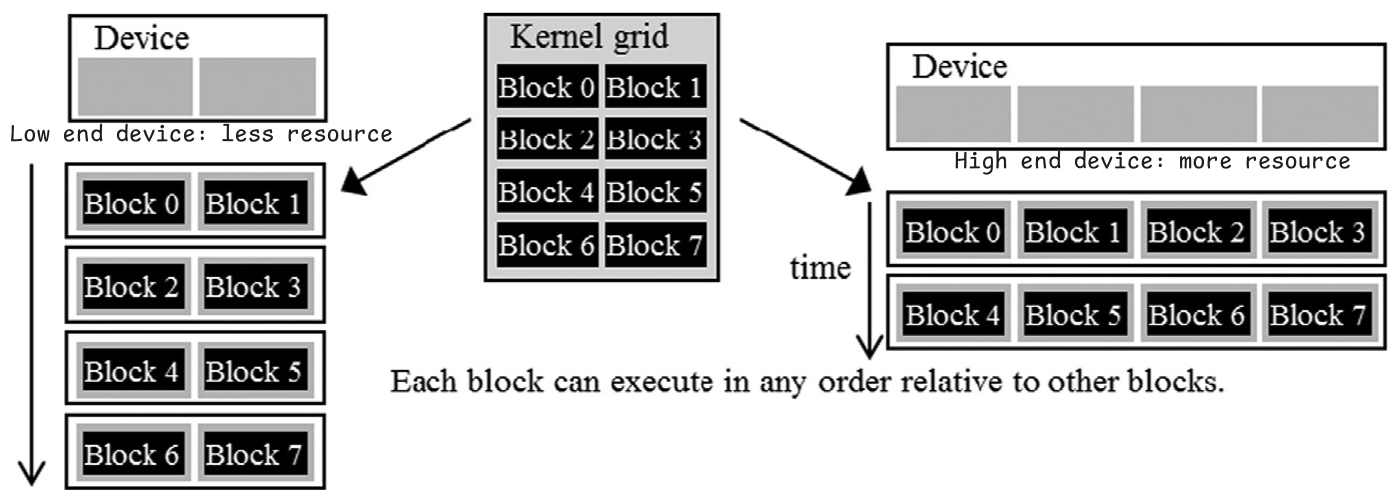
\includegraphics[width=0.9\linewidth]{Images/CompArch/Scaling.png}
          \end{center}
    \item The ability to execute the same application code with a wide range of speeds allows the production of a wide range of implementations according to the cost, power, and performance requirements of different market segments.
    \item The ability to execute the same application code on different hardware with different amounts of execution resources is referred to as \textbf{\textit{transparent scalability}}, which reduces the burden on application developers and improves the usability of applications.

\end{itemize}

\section{Warps and SIMD hardware}
\begin{itemize}
    \item One should assume that in a block, threads can execute in any order w.r.t to each other.
    \item In algorithms with phases, barrier synchronization should be used between all the threads in a block, whenever the threads must move from one phase to the other. The \textbf{correctness of executing a kernel} \textbf{\textit{shouldn't}} \textbf{depend on any assumption that threads will synchronize without the use of barrier synchronization}.
\end{itemize}

\subsection{Warps}
\begin{itemize}
    \item A block is further divided into 32-thread units called warps. \textit{The size of the warps can vary in the future.} A warp is the unit of thread scheduling in SMs.
          \begin{center}
              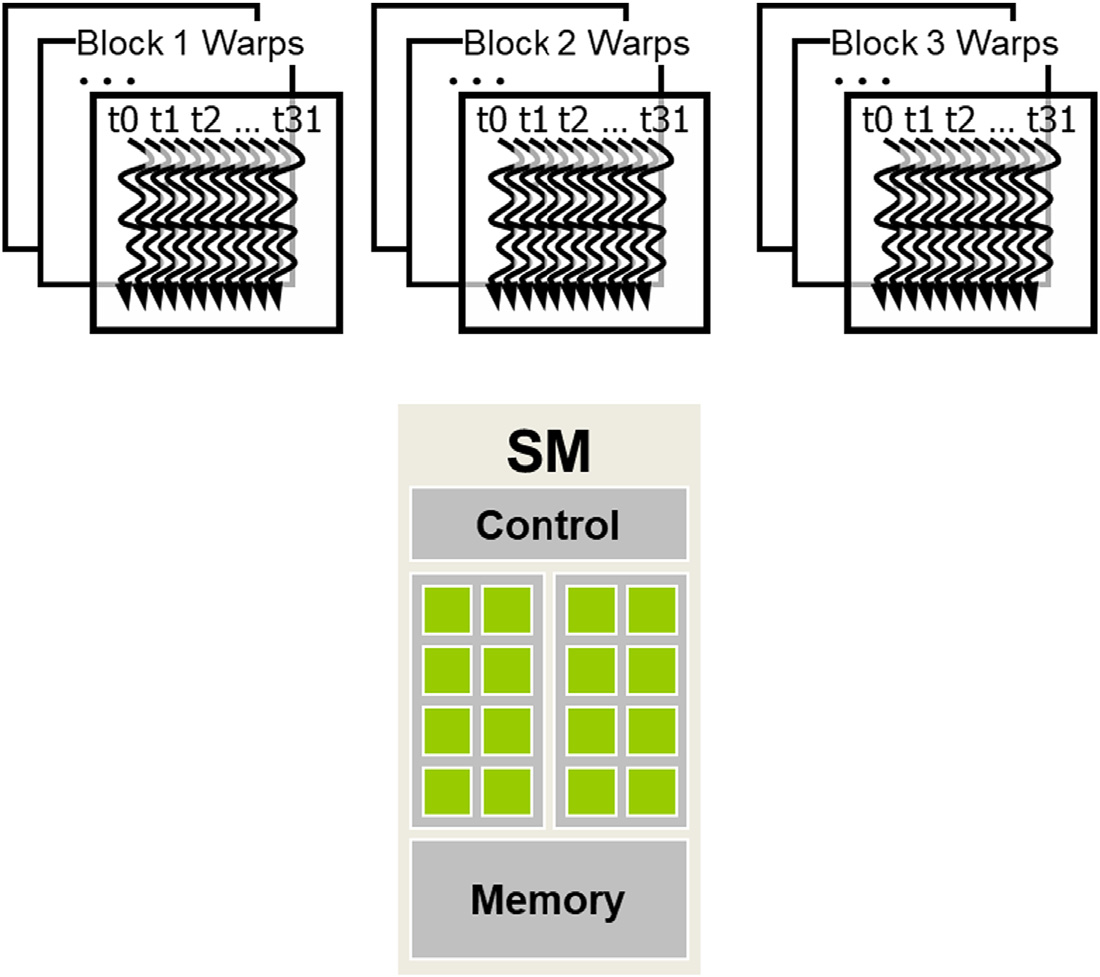
\includegraphics[width=0.8\linewidth]{Images/CompArch/Warps.png}
          \end{center}
    \item Block 1, Block 2, Block 3 - all are assigned to the single SM. Each block is further divided into warps for scheduling purposes.
          \begin{itemize}
              \item Each warp consists of 32 consecutive \texttt{threadIdx} values: threads 0 through 31 form the first warp, threads 32 through 64 the second warp etc.
              \item If each block has 256 threads, a block has 256/32 = 8 warps.
              \item With 3 blocks in the SM, there are 8 $\times$ 3 = 24 warps in the SM.
          \end{itemize}
    \item Block $\rightarrow$ Warp: Index $z$ axis, then $y$ then $x$.
          \begin{center}
              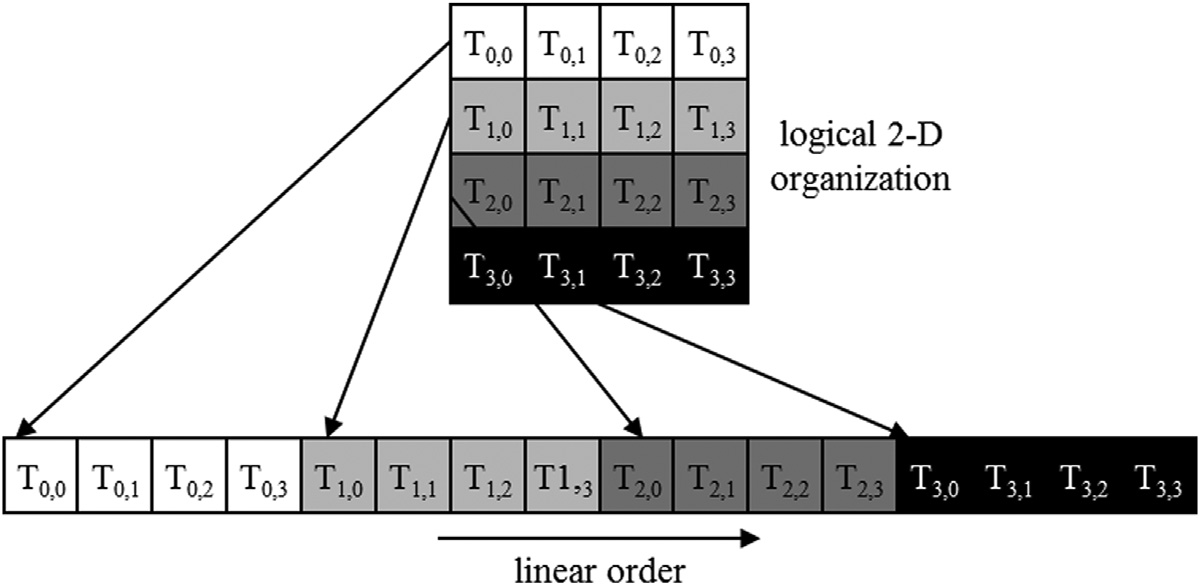
\includegraphics[width=0.7\linewidth]{Images/CompArch/Unrwrapping.png}
          \end{center}
    \item For 2D grid: $T_{\text{y,x}}$, y being \texttt{threadIdx.y} and x being \texttt{threadIdx.x}, a 2D grid is linearized by placing all the threads whose \texttt{threadIdx.y} is 0 then \texttt{threadIdx.y} is 1 and so on. Threads with the same threadIdx.y value are placed in consecutive positions in increasing threadIdx.x order.
    \item In the above figure, the 16 threads form half a warp. The warp is padded with 16 other threads to form a 32-thread warp.
    \item 2D Block with 8 $\times$ 8 threads form 2 warps of 32 threads.\\ Warp 1: $\text{T}_{0,0}$ to $\text{T}_{3,7}$\\ warp 2: $\text{T}_{4,0}$ to $\text{T}_{7,7}$
    \item 3D Block with 2 $\times$ 8 $\times$ 4 threads, form 2 warps of 32 threads. \\warp 1: $\text{T}_{0, 0, 0}$ to $\text{T}_{0,7,3}$ \\ warp 2: $\text{T}_{1,0,0}$ to $\text{T}_{1, 7, 3}$
\end{itemize}

\subsection{SIMD}
\begin{center}
    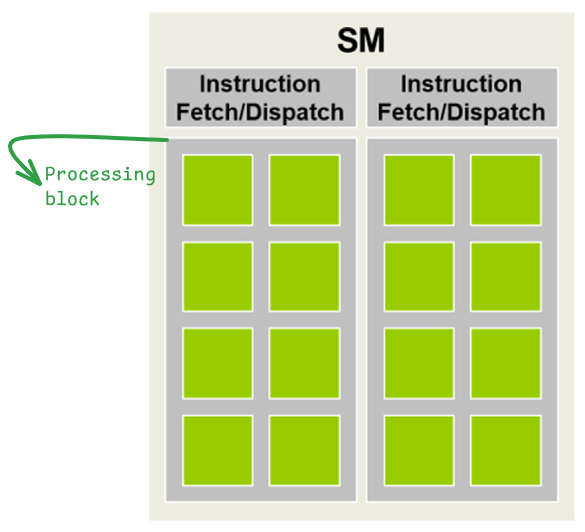
\includegraphics[width=0.3\linewidth]{Images/CompArch/SIMD_organization.png}
\end{center}
\begin{itemize}
    \item An SM is designed to execute all threads in a warp following the single-instruction, multiple-data (SIMD) model. That is, at any instant in time, one instruction is fetched and executed for all threads in the warp.
    \item As an example, in a GPU of 16 cores/SM, all the cores in a processing block share an instruction fetch/dispatch unit. \textbf{Threads in the same warp are assigned to the same processing block, which fetches the instruction for the warp and executes it for all the threads in the warp at the same time. These threads apply the same instruction to different portions of the data. Because the SIMD hardware effectively restricts all threads in a warp to execute the same instruction at any point in time, the execution behavior of a warp is often referred to as single instruction, multiple-thread.}
    \item The \textbf{advantage of SIMD} is that the \textbf{cost of the control hardware}, such as the instruction fetch/dispatch unit, \textbf{is shared across many execution units}. This design choice \textbf{allows for a smaller percentage of the hardware to be dedicated to control and a larger percentage to be dedicated to increasing arithmetic throughput}.
\end{itemize}

\subsubsection{- von Neuman Model}
\begin{center}
    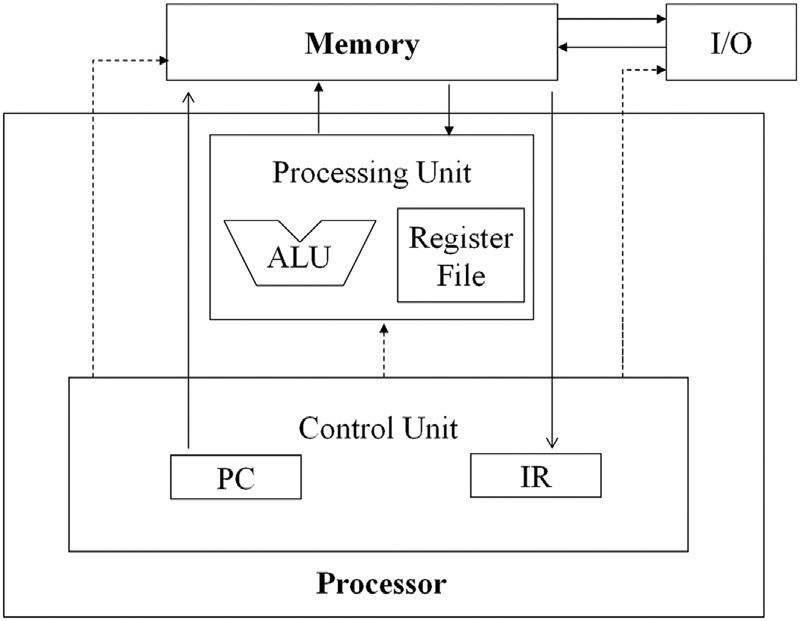
\includegraphics[width=0.4\linewidth]{Images/CompArch/neuman.png}
\end{center}
\begin{itemize}
    \item The computer has an I/O (input/output) that allows both programs and data to be provided to and generated from the system.
    \item Computer loads the program and data into memory, before executing the program. Program is a set of instructions.
    \item The \textsl{Control Unit} maintains a \textsl{Program Counter}(PC), which contains the memory address of the next instruction that is to be executed.
    \item In each \textsl{\enquote{instruction cycle}}, the \textsl{Control Unit} uses the \textsl{PC} to fetch an instruction into the \textsl{Instruction Register}(IR).
    \item The instruction bits are then examined to determine the action to be taken by all the components of the computer.
\end{itemize}

\subsubsection{- Modified von Neuman Model for SIMD}
\begin{center}
    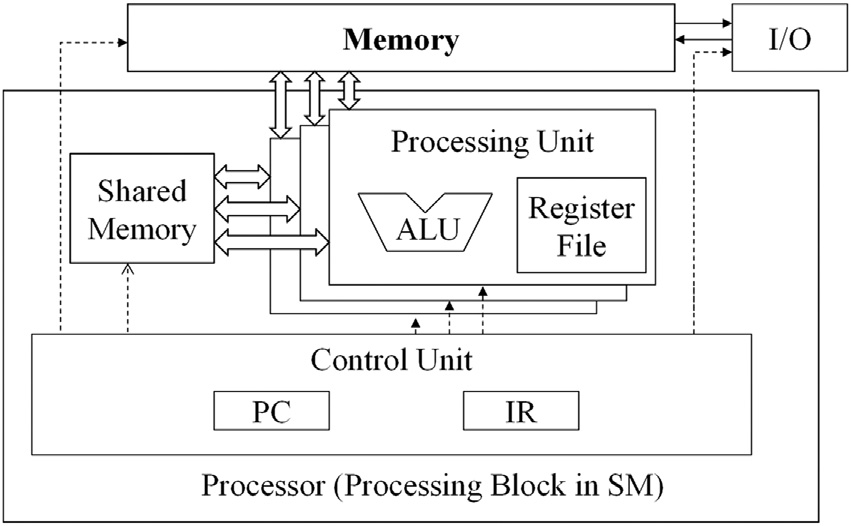
\includegraphics[width=0.5\linewidth]{Images/CompArch/neuman_simd.png}
\end{center}
\begin{itemize}
    \item Since all processing units are controlled by the same \textsl{Instruction Register} (IR) of the \textsl{Control Unit}, the only execution differences in these units are the input data (in register files) on which they operate on.
    \item This is \textsl{Single Instruction Multiple-Data} in processor design.
    \item Control units in modern processors are complex and sophisticated for fetching instructions and access instruction cache. Having multiple processing units share the same control unit can result in significant reduction in hardware manufacturing and power consumption.
\end{itemize}

\section{Control Divergence}
\textbf{SIMD provides massive performance gains when all the threads within a warp follow the same execution path, or \textit{control flow}} when working on their data.\\
For example, in an \texttt{if-else} construct, the execution works well when either all the threads follow the \texttt{if}-path or all execute the \texttt{else}-path.\\
However, when the threads in the warp take different control paths, the SIMD hardware has to take multiple passes through these paths, with one pass per each path.
\begin{itemize}
    \item When threads in the same warp follow different execution paths, we say that these threads exhibit control divergence, that is, they diverge in their execution.
    \item While the \textbf{hardware} executes the same instruction for all threads in a warp, it \textbf{selectively lets these threads take effect in only the pass that corresponds to the path that they took}, allowing every thread to appear to take its own control flow path.
    \item This preserves the independence of threads while taking advantage of the reduced cost of SIMD hardware.
    \item The cost of divergence, however, is the extra passes the hardware needs to take as well as the execution resources the inactive threads consume in each pass.
\end{itemize}
\subsubsection{- Example: \texttt{if-else-loop}}
\begin{center}
    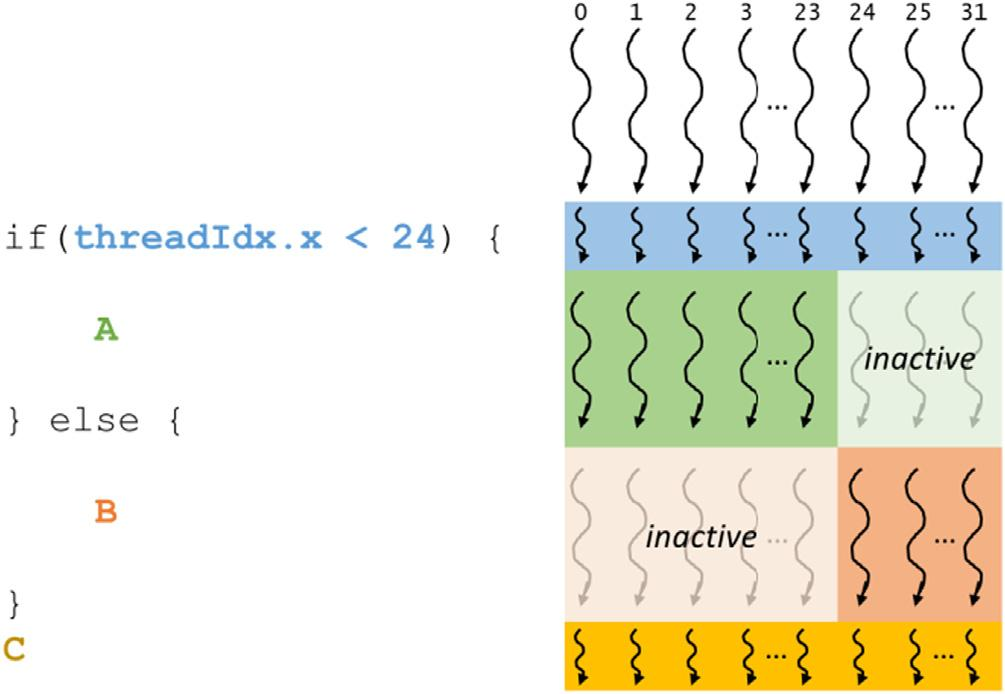
\includegraphics[width=0.6\linewidth]{Images/CompArch/control_divergence_ifelse.png}
\end{center}
\begin{itemize}

    \item First Pass:
          \subitem threads with $\texttt{threadIdx.x} < 24$ execute \texttt{A}.
          \subitem threads with  $24 < \texttt{threadIdx.x} <= 32$ are inactive.
    \item Second Pass:
          \subitem threads with  $24 < \texttt{threadIdx.x} <= 32$ execute \texttt{B}.
          \subitem threads with $\texttt{threadIdx.x} < 24$ are inactive.
    \item The threads in the warp reconverge and then execute \texttt{C}.
    \item From the Volta architecture onwards, the passes may be executed concurrently, meaning that the execution of one pass may be interleaved with the execution of another pass, known as \textit{independent thread scheduling}.
\end{itemize}

\subsubsection{- Example: \texttt{for-loop}}
\begin{center}
    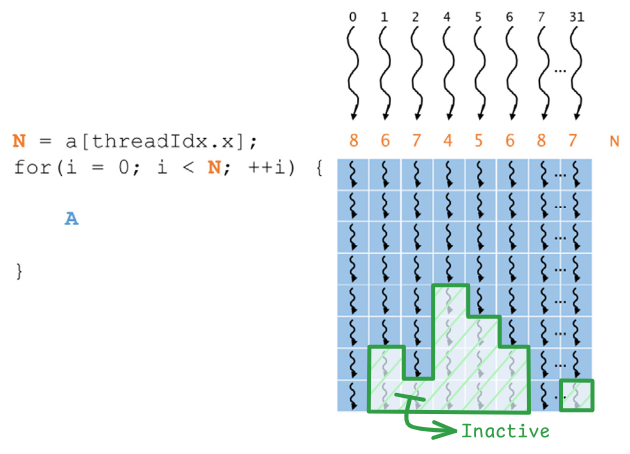
\includegraphics[width=0.5\linewidth]{Images/CompArch/control_divergence_for.png}
\end{center}

\begin{itemize}
    \item The for loop varies between 4 and 8.
    \item For the first four iterations, all threads are active and execute A.
    \item For the remaining iterations, some threads execute A, while others are inactive because they have completed their iterations.
\end{itemize}

\subsubsection{- To guess thread/control divergence}
\begin{itemize}
    \item If the decision condition is based on threadIdx values, the control statement can potentially cause thread divergence.
    \item For example, the statement \texttt{if(threadIdx.x $>$ 2) \{\dots\}} causes the threads in the first warp of a block to follow two divergent control flow paths.
          \subitem Threads 0, 1, and 2 follow a different path than that of threads 3, 4, 5, and so on.
\end{itemize}

\subsubsection{- Reasons to use control construct with thread control divergence}
\begin{itemize}
    \item To handle boundary conditions when mapping threads to data.
          \begin{itemize}

              \item \textbf{Example}: Vector length: 1003, Block size: 64 $\implies$ (1003 + 64 - 1)/64, i.e, 16 thread blocks to process the 1003 elements.
              \item 16 thread blocks $\rightarrow$ have 1024 total threads.
              \item We need to disable the last 21 threads in thread block 15 from doing work that is not expected or not allowed by the original program.
              \item The 16 blocks are partitioned into 32 warps. \textbf{Only the last warp} (i.e., the second warp in the last block) \textbf{will have control divergence.}
          \end{itemize}
    \item The performance impact of control divergence decreases as the size of the vectors being processed increases.
          \begin{itemize}
              \item For a vector length of 100, one of the four warps will have control divergence. (25\%)
              \item For a vector size of 1000, only one of the 32 warps will have control divergence. (4\%)
              \item For a vector of length 10,000, only one of the 313 warps will have control divergence. (0.3\%)
          \end{itemize}
    \item Due to the control divergence, one can not confidently assume that all the threads in the warp have the same execution timing. If all threads in a warp must complete one phase before moving to the next phase, barrier synchronization mechanism such as \texttt{\_\_syncwarp()} is to be used.
\end{itemize}

\section{Warp scheduling and latency tolerance}
When the threads are assigned to SMs, usually the number of threads exceeds the number of cores in the SM. This abundance of the warps/threads help the CUDA system to effectively schedule the warps.\\
In a warp, when the instruction that needs to be executed has to wait on the results of the previously initiated long-latency operation, the warp is not selected for execution. Instead, another warp resident in the SM is selected which is no longer waiting for the results of the previous instructions. If more than one warp is ready for execution, a priority mechanism is used to select one for execution.\\
\linebreak
This \textbf{mechanism of filling the latency time of operations from some threads with work from other threads is often called \enquote{latency tolerance}} or \enquote{latency hiding}. Warp scheduling is also used for tolerating other types of operation
latencies, such as pipelined floating-point arithmetic and branch instructions. With enough warps around, the hardware will likely find a warp to execute at any point in time, thus making full use of the execution hardware while the instructions of some warps wait for the results of these long-latency operations.

\section{Resource partitioning and occupancy}
\begin{itemize}
    \item \textbf{Occupancy}: The ratio of number of warps assigned to an SM to the maximum number of warps the SM supports.
    \item As the threads in an SM share the resources, registers and shared memory of that SM, a limited number of thread blocks can be assigned to an SM.
    \item \textsl{Example}: an Ampere A100 GPU can support maximum of:
          \subitem 32 blocks / SM.
          \subitem 64 warps / SM.
          \subitem 2048 threads / SM.
          \subitem 1024 threads / block.\\
          \linebreak
          If a grid is launched with a block size of 1024 threads (maximum allowed), the 2048 thread slots in SM are partitioned into 2 blocks. $\implies$ Each SM can accommodate 2 blocks.
          \subitem Block size: 512 $\implies$ 4 blocks / SM
          \subitem Block size: 256 $\implies$ 8 blocks / SM
          \subitem Block size: 128 $\implies$ 16 blocks / SM
          \subitem Block size: 64 $\implies$ 32 blocks / SM
    \item  The ability to dynamically partition the thread slots among blocks make SMs robust. They can either execute many blocks with few threads or few blocks with many threads.
          \subitem If fixed partition was the norm, then there would be either wasted thread slots when blocks require fewer threads than what the partition supports or fail in execution of the block when the requirement of threads is greater than supported.
\end{itemize}

\subsubsection{- Underutilization with dynamic partitioning}

\begin{enumerate}
    \item With block size of 32 threads, the SM is partitioned into 2048 / 32 = 64 blocks. But an SM can support only 32 blocks at once. Means the supported 32 blocks end up using only 1024 thread slots (32 blocks, 32 threads each). The occupancy in this case is (1024 assigned threads)/(2048 maximum threads) = 50\%. $\implies$ To utilize the thread slots in an SM fully, one needs at least 64 threads / block.
    \item When the number of maximum threads is not divisible by the block size. If a block size of 700 is selected, 2048 // 700 = 2 blocks can be created in the SM. The resulting 2048 \%700 = 648 threads are left unutilized. In this case, neither maximum thread slots nor maximum number of blocks per SM are reached. The occupancy is (1400 assigned threads) / (2048 maximum threads) = 68.4\%.
\end{enumerate}

\subsubsection{- Register resource limitation on occupancy}
For example, the Ampere A100 GPU allows a maximum of 65,636 registers per SM. To run at full capacity, each of the maximum allowed 2048 threads of SM should have enough registers, which means that each thread should not use more than (64,536 registers) / (2048 threads) = 32 registers.
\begin{itemize}
    \item For example, if a thread needs 64 registers to complete its execution successfully, the maximum number of threads that can be supported in an SM is (64,536 registers) / (64 registers / thread) = 1024 threads. In this case, the kernel can not run at full occupancy regardless of what block size is set. Instead, the occupancy will be at most 50\%.
    \item Given a scenario of a kernel that uses 31 registers / thread, and has 512 threads per block. In this case, SM will have (2048 threads) / (512 threads / block) = 4 blocks running simultaneously. These threads will use a total of (2048 threads) $\times$ (31 registers/thread) = 63488 registers $<$  register limit of 64,536.
          \begin{itemize}
              \item If only the registers / thread is changed 33, the 2048 threads in the SM will need 67,584 threads $>$ maximum allowed 64,536 registers. The CUDA runtime system might assign only 3 blocks with 512 threads/block in this case. Reducing the  total required registers to 3 blocks $\times$ 512 threads/ block $\times$ 33 registers / thread = 50,688 registers. \\ In this process, the threads / SM are reduced from 2048 to 1566 (3 $\times$ 512). That is, by using 2 automatic variables, the occupancy drops from 100\% to 75\%. This is sometimes referred as \enquote{\textbf{\textsl{Performance cliff}}}, where a slight increase in resource usage (31 registers $\rightarrow$ 33 registers) can result in significant drop in parallelism performance achieved.
          \end{itemize}
\end{itemize}

\section{Device query}
\begin{minted}{cpp}
    // Get number of devices avilable.
    int devCount;
    cudaGetDeviceCount(&devCount);
    // Device property struct.
    cudaDeviceProp devProp;
    // Get properties and statisics of first GPU.
    cudaGetDeviceProperties(&devProp, 0);
    // View device statistics and properties from the devProp object.
    // Example:
    printf("Maximum threads per block  : %d", devProp.maxThreadsPerBlock);
    printf("Clockrate of the GPU       : %d GHz", devProp.clockRate / 1e6);
    printf("Man threads in x dim       : %d", devProp.maxThreadsDim[0]);
    printf("Man threads in y dim       : %d", devProp.maxThreadsDim[1]);
    printf("Man threads in z dim       : %d", devProp.maxThreadsDim[2]);
    // And many more.

\end{minted}
\pagebreak
\section{Q \& A}
\begin{enumerate}
    \item Consider the following CUDA kernel and the corresponding host function that calls it:
          \begin{center}
              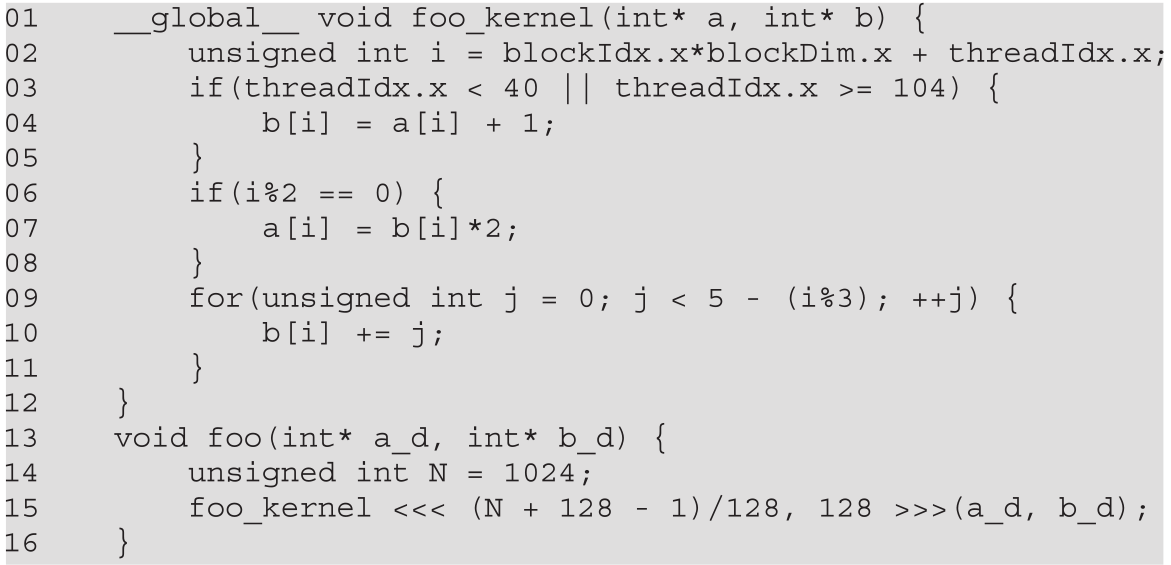
\includegraphics[width=0.7\linewidth]{Images/CompArch/qa1.png}
          \end{center}
          \begin{enumerate}
              \item What is the number of warps per block?\\
                    A: Block size = 128 $\implies$ Number of warps per block = 128/32 =\textbf{ 4}.
              \item What is the number of warps in the grid?\\
                    A: Total blocks = (1024 + 128 - 1) / 128 = 8.\\
                    Number of warps = 8 $\times$ 4 = \textbf{32}.
              \item For the statement on line 04:
                    \begin{itemize}
                        \item \textsl{How many warps in the grid are active?}
                              \\A: \textbf{In a block}, the warps which contain the elements between \texttt{threadIdx.x} $\in$ {{0,\dots,39} and {104,\dots,127}} are active. \textit{With warp size of 32, Warp 0 (0 to 31), Warp 1 (32 to 63), Warp 3 (96 to 128) are active (3 active warps).} $\implies$ 3 / 4 warps in a block are active. $\implies$ 3/4 $\times$ (32 warps in the grid) = \textbf{24 warps are active.}

                        \item \textsl{What is the SIMD efficiency (in \%) of warp 0 of block 0?}
                              \\A: In warp 0 all threads in index 0 \dots 31 are executed. Thus, the efficiency of the warp is \textbf{100\%}.
                        \item \textsl{What is the SIMD efficiency (in \%) of warp 1 of block 0?}
                              \\A: In warp 1 the threads with indices between 32 \dots 39 are executed (8 threads). The efficiency of warp 1 is (8 threads execute) / (32 threads in the warp) = \textbf{25\%}.
                        \item \textsl{What is the SIMD efficiency (in \%) of warp 3 of block 0?}
                              \\A: In warp 3 the threads with indices between 104 \dots 127 are executed (23 threads). The efficiency of warp 3 is (23 threads execute) / (32 threads in the warp) = \textbf{75\%}.
                    \end{itemize}
              \item For the statement on line 07:
                    \begin{itemize}
                        \item \textsl{How many warps in the grid are active?}
                              \\A: All the 32 warps are active as threads with even indices are found in all the warps.
                        \item \textsl{How many warps in the grid are divergent?}
                              \\A: All the 32 warps are divergent, as the even threads are distributed in all the warps. The threads with even index take the if-then path, while the threads with odd indices do not enter the if statement.
                        \item \textsl{What is the SIMD efficiency (in \%) of warp 0 of block 0?}
                              \\A: Among the 32 threads, only 16 of them are active in line 07. $\implies$ \textbf{50\% SIMD efficiency.}
                    \end{itemize}
              \item For the loop on line 09:
                    \begin{itemize}
                        \item \textsl{How many iterations have no divergence?}
                              \\A: $\min{(\texttt{5 - i\%3})} ~\equiv~ { 5 - \max{(i\%3)}} ~\equiv~ \texttt{5 - 2} = 3$. The loop reduces to:\\\texttt{for (int j = 0; j < 3; +j)}. As all the blocks execute the for loop until j $\in$ {0, 1, 2}, \textbf{3 iterations have no divergence}.
                        \item \textsl{How many iterations have divergence?}
                              \\A: $\max{(\texttt{5 - i\%3})} ~\equiv~ { 5 - \min{(i\%3)}} ~\equiv~ \texttt{5 - 0} = 5$. There are 5 iterations possible. Out of the 5, 3 are not divergent. $\implies$ \textbf{2 divergent iterations.}
                    \end{itemize}
              \item For a vector addition, assume that the vector length is 2000, each thread calculates one output element, and the thread block size is 512 threads. How many threads will be in the grid?
                    \\A: Block size : 512. To include all 2000 elements of the vector, there has to be\\ (2000 + 512 - 1) / 512 = 4 blocks. $\implies$ 4 \(\times\)512 = \textbf{2048 threads.}
              \item For the previous question, how many warps do you expect to have divergence due to the boundary check on vector length?
                    \\A: Number of warps: (2048 threads) / (32 threads per warp) = 64 warps. 63 warps cover the entire vector of 2000 elements. (63 * 32 = 2016 threads.) $\implies$ As 62 * 32 = 1984 $<$ 2000, the last (\(63^{rd}\)) warp will have divergence. \textbf{One warp with divergence.}

              \item Consider a hypothetical block with 8 threads executing a section of code before reaching a barrier. The threads require the following amount of time (in microseconds) to execute the sections: 2.0, 2.3, 3.0, 2.8, 2.4, 1.9, 2.6, and
                    2.9; they spend the rest of their time waiting for the barrier. What percentage of the threads’ total execution time is spent waiting for the barrier?
                    \\A: The maximum time required is 3.0 \(\mu\)s.\\
                    \begin{equation*}
                        \begin{aligned}
                            Time_{idle} = & \frac{1}{n}\sum_{n}^{8} max(T) - t                                                             \\
                            =             & 0.5125 \mu s. \implies \frac{100 \times 0.5125}{3} = \text{\textbf{17.08\% is spent waiting.}}
                        \end{aligned}
                    \end{equation*}
              \item A CUDA programmer says that if they launch a kernel with only 32 threads in each block, they can leave out the \texttt{\_\_syncthreads()} instruction wherever barrier synchronization is needed. Do you think this is a good idea? Explain.
                    \\A: Launching the kernel with 32 threads per block does not promise the timely execution of all the threads like the barrier synchronization does. Assuming and tweaking the block, warp size does not ensure the correctness of the execution when the execution happens in phases.
              \item If a CUDA device’s SM can take up to 1536 threads and up to 4 thread blocks, which of the following block configurations would result in the most number of threads in the SM?
                    \begin{itemize}
                        \item[a.] \textsl{128 threads per block}
                        \item[b.] \textsl{256 threads per block}
                        \item[\textcolor{ForestGreen}{c.}] \textcolor{ForestGreen}{\textsl{512 threads per block}}
                        \item[d.] \textsl{1024 threads per block}
                              \\
                              \linebreak
                              A: 1536 \% 3 = 0 \&\& 1536 / 3 = 512 \(\implies\) 3 blocks with 512 threads each yield in 100\% occupancy.
                    \end{itemize}
              \item Assume a device that allows up to 64 blocks per SM and 2048 threads per SM. Indicate which of the following assignments per SM are possible. In the cases in which it is possible, indicate the occupancy level.
                    \begin{itemize}
                        \item[a.] \textsl{8 blocks with 128 threads each}
                              \\A. 8 \(\times\) 128 = 1024 \(\implies\)Possible with Occupancy = 50\%
                        \item[b.] \textsl{16 blocks with 64 threads each}
                              \\A. 16 \(\times\) 64 = 1024 \(\implies\)Possible with Occupancy = 50\%
                        \item[c.] \textsl{32 blocks with 32 threads each}
                              \\A. 32 \(\times\) 32 = 1024 \(\implies\)Possible with Occupancy = 50\%
                        \item[d.] \textsl{64 blocks with 32 threads each}
                              \\A. 64 \(\times\) 32 = 2048 \(\implies\)Possible with Occupancy = 100\%
                        \item[e.] \textsl{32 blocks with 64 threads each}
                              \\A. 32 \(\times\) 64 = 2048 \(\implies\)Possible with Occupancy = 100\%
                    \end{itemize}
              \item Consider a GPU with the following hardware limits: 2048 threads per SM, 32 blocks per SM, and 64K (65,536) registers per SM. For each of the following kernel characteristics, specify whether the kernel can achieve full occupancy. If not, specify the limiting factor.
                    \begin{itemize}
                        \item[a.]
                              \textsl{The kernel uses 128 threads per block and 30 registers per thread.}
                              \\A. Num. of blocks= (2048 threads) / (128 threads/block) = 16 blocks \textcolor{ ForestGreen}{$<$ 32 blocks. OK.}\\
                              $\bullet$ Total registers = total threads $\times$ registers per thread. = 16 $\times$ 128 $\times$ 30 \\
                              = 61,440 $<$ 65,536 total registers \textcolor{ForestGreen}{OK.} Total occupancy with threads can be reached.
                        \item[b.]
                              \textsl{The kernel uses 32 threads per block and 29 registers per thread.}
                              \\A. Num of blocks = 2048 / 32 = 64 blocks \textcolor{Red}{ $>$ 32 blocks. NOK.}

                        \item[c.]
                              \textsl{The kernel uses 256 threads per block and 34 registers per thread.}
                              \\A. Num of blocks = 2048 / 256 = 8 blocks \textcolor{ ForestGreen}{$<$ 32 blocks. OK.}\\
                              $\bullet$ Total registers = 8 $\times$ 256 $\times$ 34 = 69632 \textcolor{Red}{ $>$ 32 blocks. NOK.}
                    \end{itemize}
              \item A student mentions that they were able to multiply two 1024 $\times$ 1024 matrices using a matrix multiplication kernel with 32 $\times$ 32 thread blocks. The student is using a CUDA device that allows up to 512 threads per block and up to 8 blocks per SM. The student further mentions that each thread in a thread block calculates one element of the result matrix. What would be your reaction and why?
                    \\ A. Total threads in a block: 32 $\times$ 32 = 1024 $>$ allowed 512 threads / block. Not possible.
          \end{enumerate}
\end{enumerate}
\pagebreak